\documentclass[a4paper,12pt]{article}
\usepackage[T1]{fontenc}
\PassOptionsToPackage{defaults=hu-min}{magyar.ldf}
\usepackage[magyar]{babel}
\usepackage[a4paper]{geometry}
\geometry{margin=2cm}
\usepackage{graphicx}
\usepackage{fancyhdr}



\pagestyle{fancy}
\fancyhf{}
\fancyhead[LE,RO]{\normalfont\normalsize\thepage}
\fancyhead[RE]{\nouppercase{\sffamily\small\leftmark}}
\fancyhead[LO]{\nouppercase{\sffamily\small\rightmark}}


\begin{document}
\title{\textsc{Webprogramozás III. Gy. \\ {\normalsize (LBT\_IM744G2)}} \\ {\normalsize Beadandó feladat dokumentáció}}
\author{Kovács Norbert \\ ANOXWJ}
\maketitle
\newpage
\tableofcontents
\newpage


\section{Weboldal koncepciója}
\subsection{Technikai részletek}
A beadandó feladatot, az órán is alkalmazott \textit{xampp} szerverrel kívánom megvalósítani, \textit{apache netbeans} fejlesztőkörnyezettel. A Mysql kezelését a videóban is használt, \textit{phpmyadmin} oldalon intézem. Nem fontos részlet, a megvalósítás szempontjából, de a Windows operációs rendszer, virtuális gépként fut.

\begin{center}
	\textit{{\footnotesize Követelmény: ,,A beadandó feladat PHP MVC keretrendszerben készül!''}}
\end{center}

\begin{itemize}
	\item OS: Windows 10 Pro (21H1)
	\item Kernel: 10.0.19041.1023
	\item Mysql: 10.4.19-MariaDB
	\item PHP: 8.0.6
	\item Apache Netbeans IDE: 12.3
	\item CodeIgniter: 3.1.11
\end{itemize}

\subsection{Elképzelés}
A weboldal egy \textit{fiktív} szervezet köré épül, aminek a feladata  az \textit{állategészségügy}, és \textit{állatvédelem}. A fiktív szervezetnek több városban lesznek épületei országszerte. Egy városban több különféle épület is tartozhat a szervezethez. Például tartozhat állatmenhely, ahol kutyákat tárolnak, állatorvosi rendelő vagy éppen raktárépület.

Hasonlóképpen az egyetemi példafeladathoz, ahol
\begin{center}
	Kampusz -> Épület -> Terem \\[0.5cm]
	Pl.: Eger -> C épület -> 124-es terem,
\end{center}
felosztás található, itt is három rétegre kívánom felosztani a problémát, mégpedig:
\begin{center}
	Régió -> Épület -> Iroda\\[0.5cm]
	Pl.: Miskolc -> Orvosi rendelő -> 1-es vizsgáló
\end{center}

A fiktív szervezetet, az előző beadandóm állatotthonából fejlesztem tovább, részben idő spórolás céljából, részben a hasonló koncepcióból adódóan.\\
Szervezet neve: \textbf{Kék mancs}.


\section{Adatbázis tervezése}
Az adatbázis során a következőkben tervezett entitásokon kívül, még számos entitással lehetne bővíteni az adatbázist, viszont így is 7 tábla születik, a kapcsoló tábla figyelembe vétele nélkül.


\subsection{ER modell}
A pluszba kapott egyedi azonosító mezőket, és az idegen kulcsokat nem tüntetjük fel a tervezés során.

\begin{enumerate}
	\item Régió \\
	Egy Régió eltárolásához, elegendő a régió \textit{neve} (ami gyakorlatilag a város neve), és egy \textit{leírás} mező.
	
	\item Épület \\
	Az épület entitás kapcsán, elég tárolnunk az épület \textit{nevét}, és \textit{leírását}.
	
	\item Iroda \\
	Egy épület alegysége, az iroda entitás lesz. Elegendő tárolnunk a \textit{nevét}, és a \textit{kapacitását}.
	
	\item Kutya \\
	Egy kutya esetén, tárolnunk kell a \textit{nevét}, \textit{leírását}, \textit{születési évét}, \textit{nemét} és egy hozzá tartozó \textit{képet}. A kutya \textit{életkora}, származtatott tulajdonság lesz.
	
	\item Alkalmazott \\
	Az alkalmazottak esetén, tároljuk el az alkalmazott teljes \textit{nevét}.
	
	\item Feladatkör \\
	A feladatkörnek \textit{tároljuk} a nevét és \textit{leírását}.
	
	\item Munkakör \\
	A munkakör kapcsán, tároljuk a \textit{nevét}, a \textit{leírását}, és a hozzá tartozó \textit{fizetést}.
\end{enumerate}

\begin{center}
	\includegraphics[width = 17cm]{"draw_io/SQL_tervezés.png"} \\
	{\small Az ER modell}
\end{center}

\begin{center}
	\textit{{\small Követelmény: ,,A megvalósítandó projekthez tartozó adatmodell legalább 5 forgalmi adattáblát tartalmaz (a külső modulok által használt táblákon kívül). Az adatmodell legalább 3. normálformában van és modellben megtalálható az egy-több, valamint a több-több típusú kapcsolat is. A technikai okokból létrehozott táblák (kapcsolótáblák) nem tekintendőek forgalmi táblának.''}}
\end{center}
\newpage
\subsection{Relációs adatmodell}
Az elkészült modell alapján, a következő táblák jöttek létre.
\begin{center}
	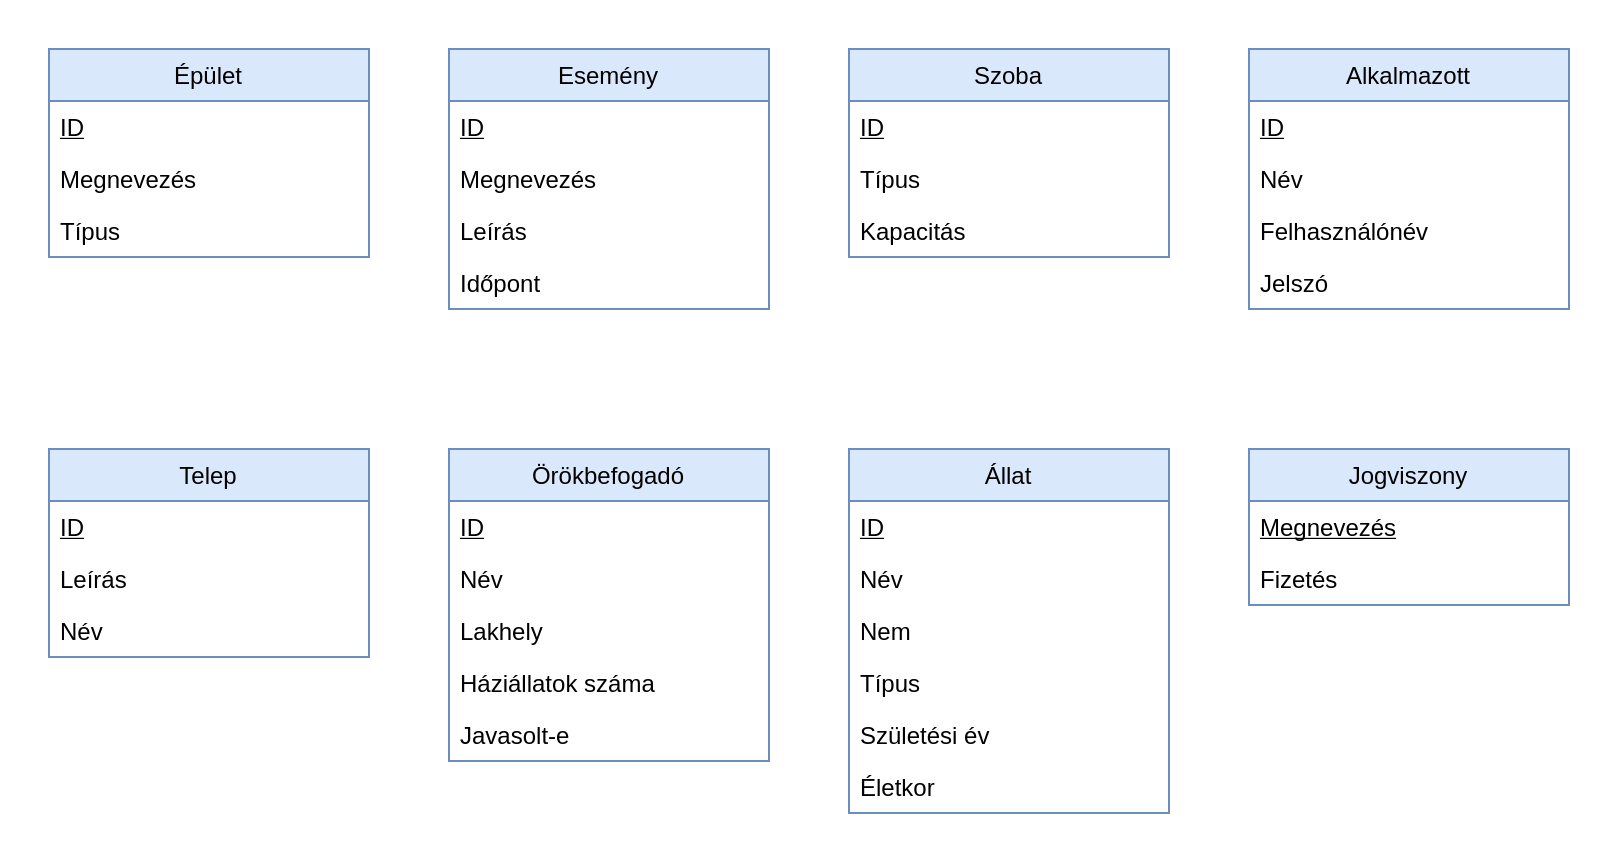
\includegraphics[width = 15cm]{"draw_io/SQL_Táblák.png"} \\
	{\small Az ER modell}
\end{center}
Hozzuk létre a szükséges kapcsolótáblákat, és illesszük be az idegen kulcsokat, majd jelöljük a kapcsolatokat.

\begin{center}
	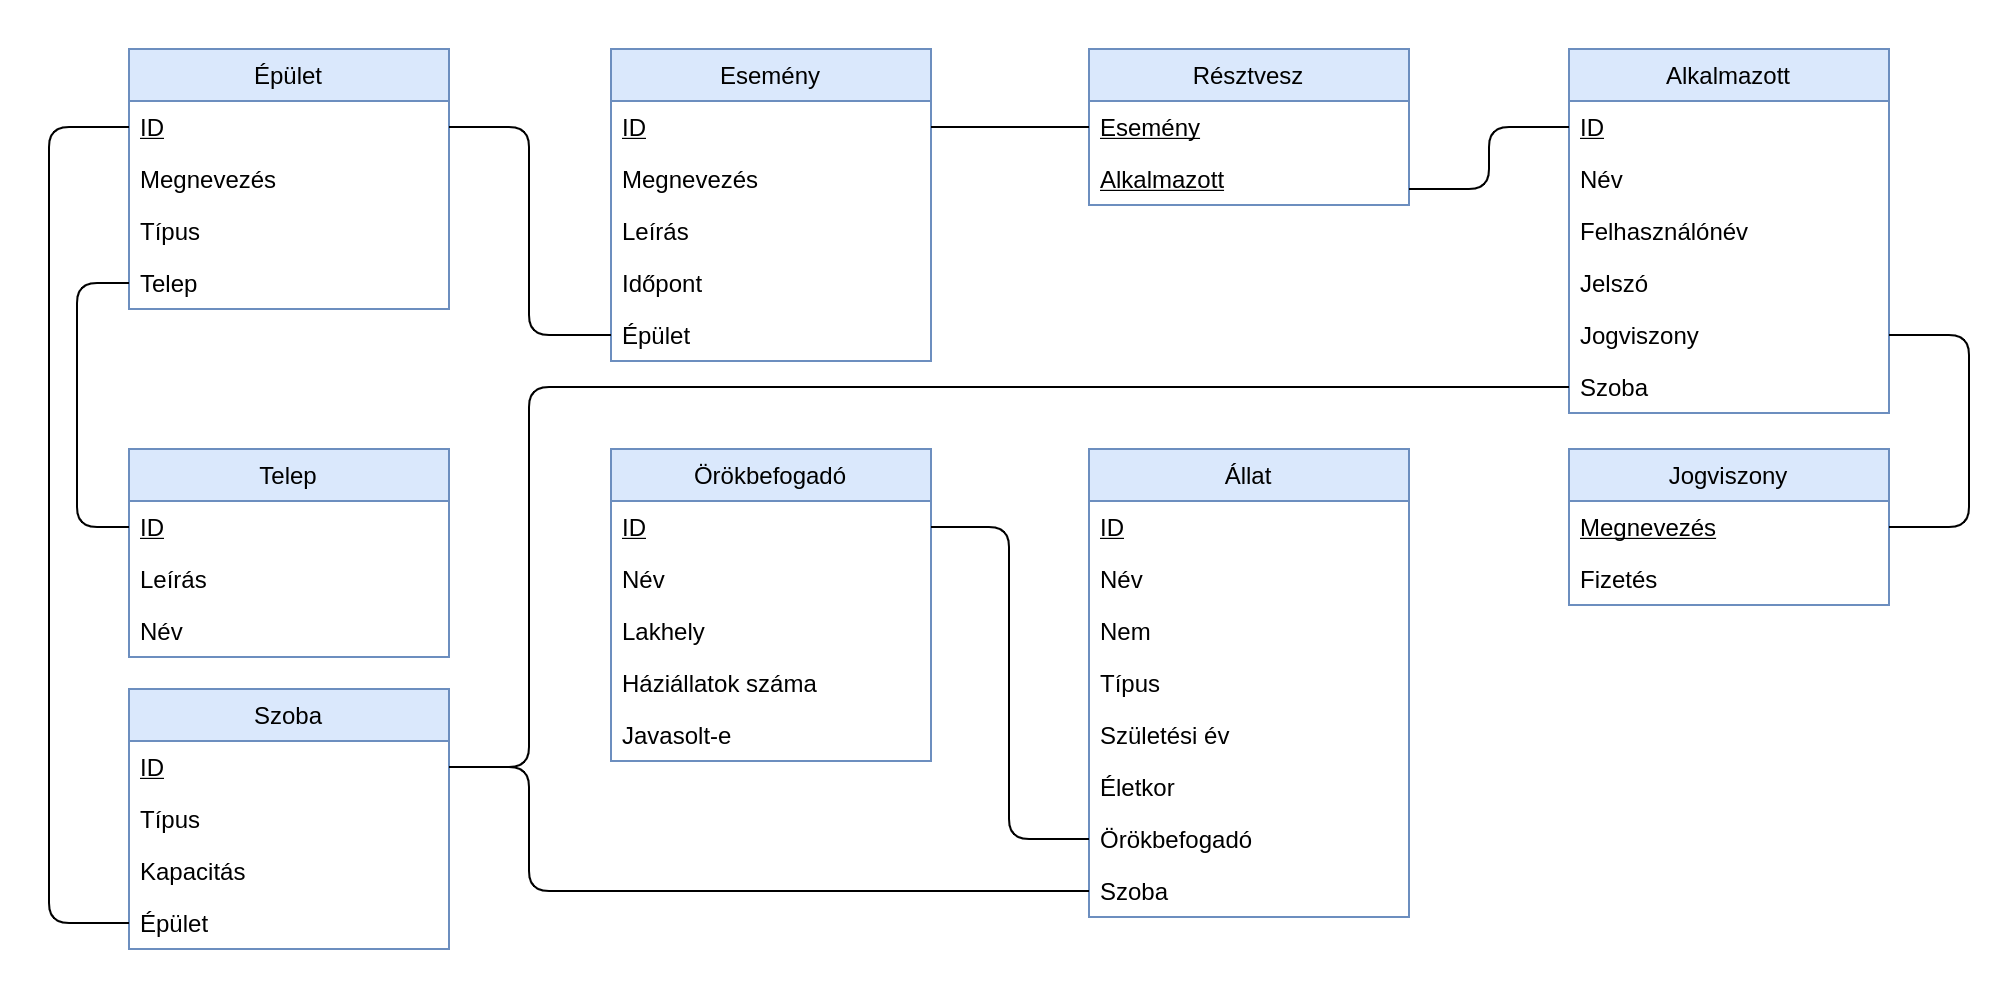
\includegraphics[width = 18cm]{"draw_io/SQL_Táblák_kapcsolatok.png"} \\
	{\small Az ER modell a kapcsolatokkal}
\end{center}
\subsection{SQL parancsok}
Az SQL parancsok megtalálhatóak az \textit{application/create.sql} fájlban.
\section{Összefoglaló}


\end{document}
